\begin{tikzpicture}
\tikzstyle{eng-step} = [draw, thick, align=center, minimum width=1cm, minimum height=1cm]


%%% Switch %%%

\coordinate (s) at (-1.0, 0);
\node[eng-step, rotate=270] (switch)  at (0, 0) {\Large \faSitemap};

%%% Controllers %%%

\node[eng-step] (c1)  at (-2.25, 1) {\Large$\mathcal{C}_1$};
\node[eng-step] (c2) at ( -2.25, -1) {\Large$\mathcal{C}_2$};
\coordinate (c) at (-4.0, 0);

%%%% Plant %%%

\node[eng-step] (plant)     at (2.5,0) {\Large$\mathcal{P}$};
\coordinate (p1) at (-4.5, -2);
\coordinate (p2) at (4.0, -2);

%%%%%%%%%%%%%%%
%%%% ARROWS %%%
%%%%%%%%%%%%%%%

\draw[-latex,thick] (c1.east)  -| ([yshift=2.5mm]s) -- ([yshift=2.5mm]switch.south);
\draw[-latex,thick] (c2.east)  -| ([yshift=-2.5mm]s) -- ([yshift=-2.5mm]switch.south);

\draw[-latex,thick] (switch.north) to (plant.west);

\draw[-,thick] (plant.east)  -| (p2) -- (p1) |- (c);

\draw[-latex,thick] (c)  -| (-3.5, 1) -- (c1.west);
\draw[-latex,thick] (c)  -| (-3.5, -1) -- (c2.west);

\end{tikzpicture}
